%cSpell:ignore Erol,Sezgin,fancyhdr, hheadheighti,hheadsepi,hfootheighti,graphicx, hfootskipi, Gavrilita, Mihail, AMOO, totalheight, keepaspectratio,UML's, kata, codewars, OOAD, COFFE,ERLANG,caml, kotlin,haskel, ruby, superclass, 
\documentclass[12pt]{article}
%\usepackage[english]{babel}
%actually it works without this package//// cuz it is in english by default... it might be useful //// but not here
% \usepackage{natbib}
% \usepackage{biblatex}

% \usepackage[backend=biber]{biblatex}

%\usepackage{url}
%idk what for it is here, it is not what it seems to be, fuck it
%%\usepackage[document]{ragged2e} 
%%to justify
% i dont use it anymore
\usepackage[utf8]{inputenc}
%%%\usepackage{amsmath}
%%useless for this report... it's for math stuff
\usepackage{graphicx}
%This package enables the user to the importation of graphics into a .tex file and, apart from the usual sizing and rotational facilities, also enables the user to crop or trim an image as desired (e.g., to get rid of surrounding blank margins). The graphicx package is useful if you need to use only a part of a complete image. 
\graphicspath{{images/}}
%% includes pics inside image folder
\usepackage{parskip}
%%this shit . In the document body, don't use \parskip but a blank line to separate paragraphs.there's normally no need to add manual line breaks (\\) in the text.

\usepackage{vmargin}
%%LaTeX package which introduces paper sizes and provides macros for setting document margins. 
\usepackage{enumerate} 
%enumeration of elements  
\usepackage{caption}
%%this is for figures
\usepackage{float}
%% to position exactly the figure 
\usepackage{fancyhdr}
%%To customize the footer and header in your document first import the package fancyhdr with 
% \addbibresource{lab4.bib}
% \bibliography{my_bibliography.bib} 
\PassOptionsToPackage{hyphens}{url}\usepackage{hyperref}
\hypersetup{
    colorlinks=true,
    linkcolor=blue,
    filecolor=magenta,      
    urlcolor=cyan,
}

\renewcommand{\theenumii}{\arabic{enumii}}
\setmarginsrb{3 cm}{2.5 cm}{3 cm}{2.5 cm}{1 cm}{1.5 cm}{1 cm}{1.5 cm}
%%\setmarginsrb{hleftmargini}{htopmargini}{hrightmargini}{hbottommargini}% {hheadheighti}{hheadsepi}{hfootheighti}{hfootskipi
\title{DB Laboratory 4}								
\author{Sezgin E}							
\makeatletter
%%The \makeatletter command temporarily defines »@« as a normal character to enable changes to internal LaTeX macros outside packages (STY) or classes (CLS).
\let\thetitle\@title
%%\let allows you to copy the content of a command into a new command.
\let\theauthor\@author
%%Thus \let\foo\bar defines \foo to have the value that \bar had at the point of definition.
\makeatother
% With \makeatother this process is reversed and the »@« is set to its original character category (other). The »@« is used to protect the internal LaTeX macros. Hence you should be very careful when using these two commands.
\pagestyle{fancy}
%%After that, the "fancy" style is set by \pagestyle{fancy}
\fancyhf{}
%%The command \fancyhf{} clears the header and footer, otherwise the elements of the default "plain" page style will appear. 
\rhead{\theauthor}
%%Prints the text included inside the braces on the right side of the header. 
\lhead{\thetitle}
%%Prints the text set inside the braces on the left side of the header.
\cfoot{\thepage}
%%\cfoot{Page \thepage}  Prints the word "Page" and next the page number which is automatically set by \thepage on the center of the footer. 
        
\begin{document}
        
        %%%%%%%%%%%%%%%%%%%%%%%%%%%%%%%%%%%%%%%%%%%%%%%%%%%%%%%%%%%%%%%%%%%%
        
        \begin{titlepage}
                \centering
                \vspace*{0.5 cm}
                
\includegraphics[scale = 0.11]{LOGO_UTM.jpg}\\[1.0 cm]	% University Logo
                %% Importing a graphic is done by using the command \includegraphics[key1=...,key2=...,etc.]{filename} Optional parameters—called “keys”—enable the figure to be resized, rotated, cropped, trimmed, etc. These keys and their functions are listed below. 
                %• scale = number — a magnification factor 
                %• width = length — the width to which the figure should be scaled1
                %• height = length — the height to which the figure should be scaled2 
                %• totalheight = length — height plus depth of figure (to be used if figure is rotated) 
                %• keepaspectratio = true/false — maintains the height/width ratio 
                %• angle = number — angle (in degrees) by which the figure is to be rotated counterclockwise 
                %• origin = location3 — the point about which rotation is to occur %• draft = true/false — prevents figure from being imported, but created a named box with the dimensions of the figure (this option is used to speed up processing) 
                %• clip = true/false — excludes whatever is outside the bounding box 
                \textsc{\LARGE Technical University of Moldova}\\[2.0 cm]%%\textsc{example text} will display the example text as small caps. All of the letters will be capitalized/uppercase, but they are going to be similar in size to a lowercase letter.	
                % University Name
                \textsc{\Large 01.11.2018}\\[0.5 cm]		% Course Code

                \rule{\linewidth}{0.2 mm} \\[0.4 cm]
                %%The \rule command in normal use produces a simple black box: \rule[raise]{width}{thickness} This is useful for drawing vertical and horizontal lines.

                { \huge \bfseries \thetitle}\\
                %%Anyway, the \bfseries bold the rest of my document, even though I'm using curly braces.
                \rule{\linewidth}{0.2 mm} \\[1.5 cm]
                
                \begin{minipage}{0.4\textwidth}
                        \begin{flushleft} \large
                                \emph{Submitted To:}\\
                                Maria Cojanu\\
                %%If you want to emphasize a word or some text, use \emph. Don't just make the text italic or bold. If needed, you may change the behavior of \emph whenever you wish in the preamble and the whole document will be adjusted accordingly.
                Asst. Univ.\\
                Computer Science Department\\
                            \end{flushleft}
                            \end{minipage}~
                            \begin{minipage}{0.4\textwidth}
                
                            \begin{flushright} \large
                            \emph{Submitted By :} \\
                            Sezgin Erol\\
                
                Group FAF-161\\
                Semester 1\\
                    \end{flushright}
                
                \end{minipage}\\[2 cm]
                
                \vfill Chisinau 2018\\  
        \end{titlepage}
        
        %%%%%%%%%%%%%%%%%%%%%%%%%%%%%%%%%%%%%%%%%%%%%%%%%%%%%%%%%%%%%%%%%%%%
        \pagebreak
        %\tableofcontents
        \subsection*{ General purpose:}
        \subsubsection*{ Learn about SQL Query Language}
        
        \subsection*{Tasks:}
        \begin{itemize}
                \item Answer Questions at the end of Chapter 4;
                \item Solve ex. 1 at the end of Chapter 4;
                \item Create SQL Queries onto database which name is "universitatea" to solve tasks according to the variant  ;
                
        \end{itemize}
        \subsection*{Answers to Questions:}
        \begin{enumerate}
                \item What features does SQL Transact-SQL Query Editor offer?
                \begin{itemize}
                        
                        \item It lets us write sql queries and execute them specifying the desirable database.
                        \item provides user with autocomplete and error checking subroutine.
                        \item Built in Debugging system.

                \end{itemize}
                
                \item What do DDL, DML, DCL and TCL mean?
                \begin{itemize}
                        \item  Data Definition Language consists of the SQL commands that can be used to define the database schema. It simply deals with descriptions of the database schema and is used to create and modify the structure of database objects in database.
                
                
                
                \item  DDL commands:
                \begin{itemize}                 
                        \item COMMENT 
                        \item RENAME 
                        \item ALTER 
                        \item TRUNCATE 
                        \item DROP 
                \end{itemize}
                \item  DML commands:
                \begin{itemize}                 
                        \item UPDATE  
                        \item INSERT  
                        \item SELECT  
                        \item DELETE  
                \end{itemize}
                \item  TCL  commands:
                \begin{itemize}                 
                        \item SAVEPOINT    
                        \item REVOKE     
                \end{itemize}
                \item  DCL   commands:   
                \begin{itemize}                 
                        \item GRANT    
                        \item ROLLBACK   
                        \item COMMIT    
                \end{itemize}
                \end{itemize}
                \item Select instruction syntax:\cite{MSSQL_}
                \begin{figure}[H]
                        \centering
                        \includegraphics[width=.95\textwidth]{img.png}
                        \caption{Full Select instruction syntax for MSSQL}
                \end{figure}
                \vspace{0.5 cm}
                \item JOIN in MSSQL
                \begin{itemize}                 
                        \item A JOIN clause is used to combine rows from two or more tables, based on a related column between them.

                        Here are the different types of the JOINs in SQL:
                        \begin{itemize} 
                                \item (INNER) JOIN: Returns records that have matching values in both tables
                                \item LEFT (OUTER) JOIN: Return all records from the left table, and the matched records from the right table
                                \item RIGHT (OUTER) JOIN: Return all records from the right table, and the matched records from the left table
                                \item FULL (OUTER) JOIN: Return all records when there is a match in either left or right table
                        \end{itemize}
                \end{itemize}
                \item How to limit results from SQL queries:
                \begin{itemize}                 
                        \item The SELECT TOP clause is used to specify the number of records to return.   
                \end{itemize}
                
        \end{enumerate}


        \subsection*{Task Realization:}

        \begin{figure}[H]
                \centering
                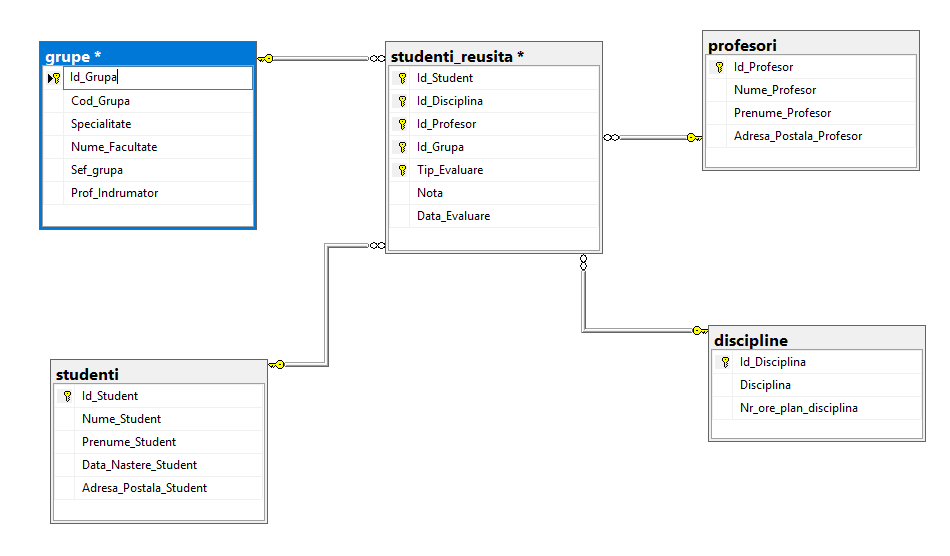
\includegraphics[width=.75\textwidth]{img1.png}
                \caption{Aflafi toate datele despre grupele de studii de la facultate}
        \end{figure}
        \vspace{0.5 cm}
        
        \begin{figure}[H]
                \centering
                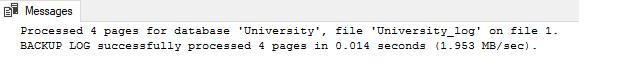
\includegraphics[width=.95\textwidth]{img2.png}
                \caption{Sa se obtina lista disciplinelor in ordine descrescatoare a numarului de ore.}
        \end{figure}
        \vspace{0.5 cm}

        
        \begin{figure}[H]
                \centering
                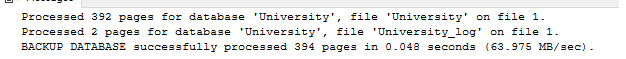
\includegraphics[width=1\textwidth]{img3.png}
                \caption{Aflati cursurile (Disciplina) predate de fiecare profesor (NumeProfesor, PrenumeProfesor) sortate descrescator dupa nume apoi prenume.}
        \end{figure}
        \vspace{0.5 cm}

        
        \begin{figure}[H]
                \centering
                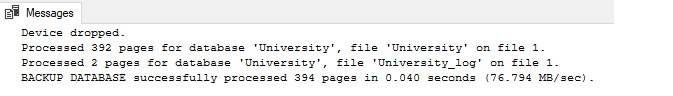
\includegraphics[width=.75\textwidth]{img4.png}
                \caption{Afi~ati care dintre discipline au denumirea formata din mai mult de 20 de caractere? }
        \end{figure}
        \vspace{0.5 cm}

        \begin{figure}[H]
                \centering
                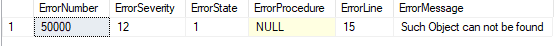
\includegraphics[width=1\textwidth]{img5.png}
                \caption{Sa se afiseze lista studentilor al caror nume se termina in ,,u" }
        \end{figure}
        \vspace{0.5 cm}

        \begin{figure}[H]
                \centering
                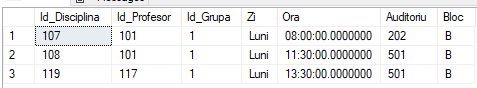
\includegraphics[width=.5\textwidth]{img6.png}
                \caption{Afi~ati numele ~i prenumele primilor 5 studenti, care au obtinut note in ordine descrescatoare la al doilea test de la disciplina Baze de date. Sa se foloseasca optiunea TOP ... WITH TIES.}
        \end{figure}
        \vspace{0.5 cm}

        \begin{figure}[H]
                \centering
                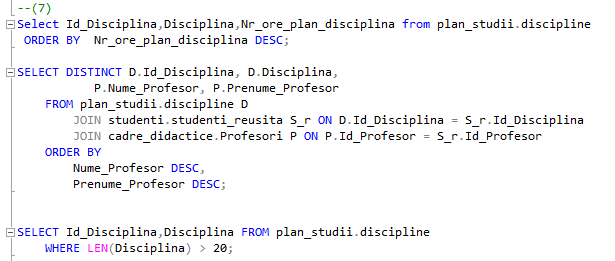
\includegraphics[width=.25\textwidth]{img7.png}
                \caption{in ce grupa (CodGrupa) invata studentii care locuiesc pe strada 31 August?  }
        \end{figure}
        \vspace{0.5 cm}

        \begin{figure}[H]
                \centering
                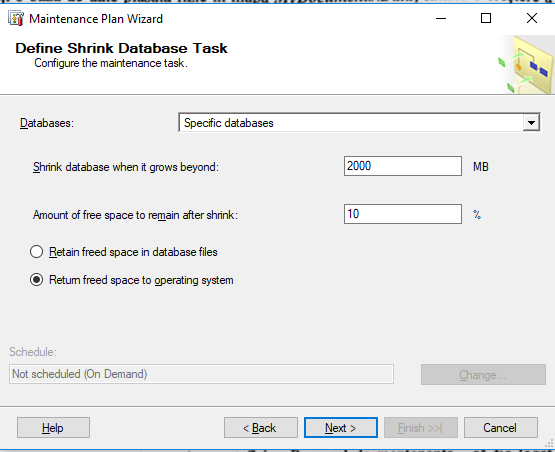
\includegraphics[width=.9\textwidth]{img9.png}
                \caption{Gasiti numele, adresa studentilor si codul disciplinei la care studentii au avut eel putin o nota mai mare decat 8 in 2018.}
        \end{figure}
        \vspace{0.5 cm}

        \begin{figure}[H]
                \centering
                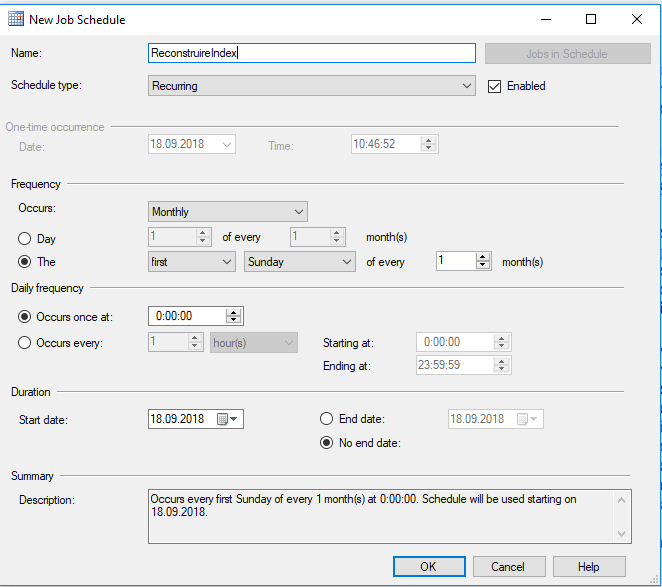
\includegraphics[width=.55\textwidth]{img10.png}
                \caption{Gasiti studentii (numele, prenumele), care au obtinut la disciplina Baze de date (examen), in anul 2018, vreo nota mai mica de 8 si mai mare ca 4.}
        \end{figure}
        \vspace{0.5 cm}

        \begin{figure}[H]
                \centering
                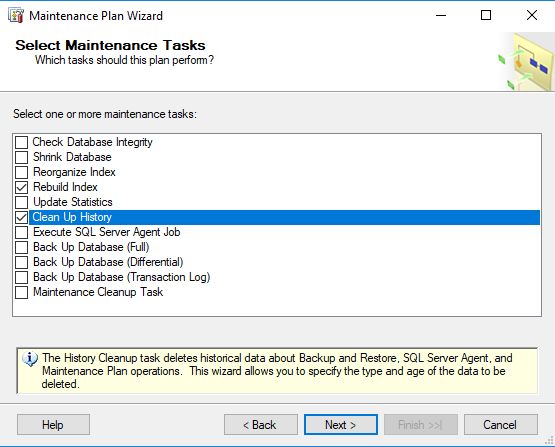
\includegraphics[width=.65\textwidth]{img11.png}
                \caption{Furnizati numele si prenumele profesorilor, care au predat disciplina Baze de date, in 2018, ~i au evaluat vreun student cu nota nesatisracatoare la reu~ita curenta.  }
        \end{figure}
        \vspace{0.5 cm}

        \begin{figure}[H]
                \centering
                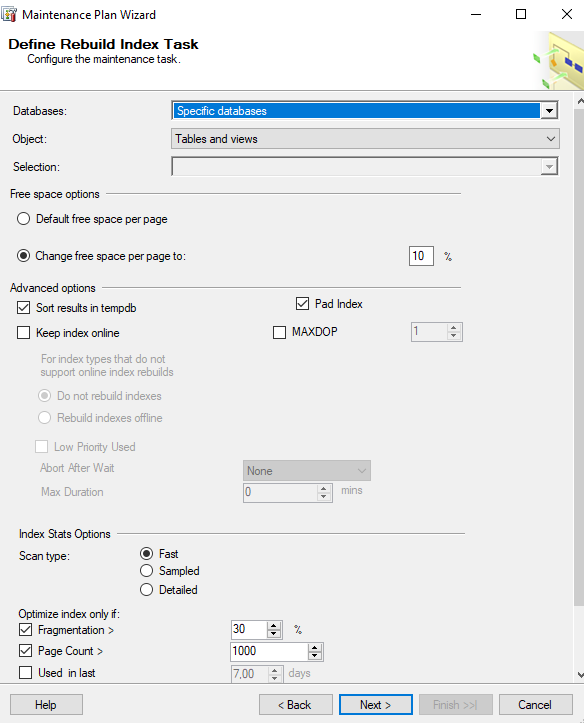
\includegraphics[width=.95\textwidth]{img12.png}
                \caption{Furnizati, in evidenta academica (reusita) a studentilor cu prenumele Alex, urmatoarele date: numele, prenumele, denumirea disciplinei, notele (inclusiv la probele intermediare) si anul la care au sustinut. }
        \end{figure}
        \vspace{0.5 cm}

        \begin{figure}[H]
                \centering
                \includegraphics[width=.85\textwidth]{img13.png}
                \caption{Aflati cursurile urmate de catre studentul Florea loan.}
        \end{figure}
        \vspace{0.5 cm}

        \begin{figure}[H]
                \centering
                \includegraphics[width=.85\textwidth]{img14.png}
                \caption{Aflati numele si prenumele studentilor, precum ~i cursurile promovate cu note mai mari de 8 la examen.}
        \end{figure}
        \vspace{0.5 cm}

        \begin{figure}[H]
                \centering
                \includegraphics[width=.37\textwidth]{img24.png}
                \caption{Sa se afi~ase lista disciplinelor (Disciplina) predate de eel putin doi profesori }
        \end{figure}
        \vspace{0.5 cm}

        \begin{figure}[H]
                \centering
                \includegraphics[width=.38\textwidth]{img25.png}
                \caption{in ce grupe de studii (CodGrupa) figureaza mai mult de 24 de studenti?  }
        \end{figure}
        \vspace{0.5 cm}

        \begin{figure}[H]
                \centering
                \includegraphics[width=.32\textwidth]{img26.png}
                \caption{Gasiti numele, prenumele ~i adresele studentilor si ale profesorilor care locuiesc pe strada 31 August.  }
        \end{figure}
        \vspace{0.5 cm}

        \begin{figure}[H]
                \centering
                \includegraphics[width=.3\textwidth]{img37.png}
                \caption{Gasiti disciplina sustinuta de studenti cu nota medie (la examen) cea mai inalta.}
        \end{figure}
        \vspace{0.5 cm}

        \newpage 
        \subsection*{Conclusion}
        During This lab work i find out how to write SQL Queries in Transact SQL. I Also trained how to make correct JOINs, GROUP BYs ans SubQueries. Also I familiarized With SQL Language.
        \cite{SQLServerManagementStudio}
        

 
\medskip
 
\begin{thebibliography}{9}
\bibitem{SQLServerManagementStudio} 
SQL Server Management Studio 2017, Tutorials for Lab 4

\bibitem{MSSQL_} 
MSSQL Official Documentation
\url{https://docs.microsoft.com/en-us/sql/t-sql/queries/select-transact-sql?view=sql-server-2017}
\end{thebibliography}
                
\end{document}